% =====================================================================
%  ARTIGO -- Astronomia (AST0001), 2026/2
%  Sicrano da Silva -- Laboratório de dados 1
%  Exemplo preenchido do modelo da disciplina.
% =====================================================================

\documentclass[10pt,a4paper,twocolumn]{article}

% ---------------------------------------------------------------- pacotes
\usepackage[utf8]{inputenc}
\usepackage[T1]{fontenc}
\usepackage[brazil]{babel}
\usepackage{amsmath,amssymb}
\let\Bbbk\relax                    % evita choque entre amssymb e newtxmath
\usepackage{newtxtext,newtxmath}   % tipografia de periódico (Times)
\usepackage{microtype}
\usepackage[a4paper,top=2.4cm,bottom=2.2cm,left=1.9cm,right=1.9cm,
            columnsep=0.7cm]{geometry}
\usepackage{graphicx}
\usepackage{booktabs}
\usepackage{siunitx}
\usepackage{caption}
\usepackage{titlesec}
\usepackage{fancyhdr}
\usepackage{xcolor}
\usepackage[colorlinks=true,linkcolor=udescverde,citecolor=udescverde,
            urlcolor=udescverde]{hyperref}

\definecolor{udescverde}{HTML}{1B6B3A}
\definecolor{cinza}{HTML}{5A5A5A}

\sisetup{output-decimal-marker={,}, per-mode=symbol}

% --------------------------------------------------- estilo das seções
\captionsetup{font=small,labelfont={bf,color=udescverde},labelsep=period}
\titleformat{\section}{\normalfont\bfseries\color{udescverde}}
            {\thesection.}{0.5em}{\MakeUppercase}
\titleformat{\subsection}{\normalfont\bfseries\itshape}{\thesubsection.}{0.5em}{}
\titlespacing*{\section}{0pt}{1.6ex}{0.8ex}
\setlength{\parindent}{1.2em}

% ---------------------------------------------------- PREENCHA AQUI
\newcommand{\titulo}{A densidade estelar da vizinhança solar medida com
2000 paralaxes do \textit{Gaia}}
\newcommand{\aluno}{Sicrano da Silva}
\newcommand{\email}{sicrano.silva@edu.udesc.br}
\newcommand{\tituloCurto}{Densidade estelar da vizinhança solar}
\newcommand{\semestre}{2026/2}
% -------------------------------------------------------------------

% ------------------------------------------------ cabeçalho das páginas
\pagestyle{fancy}
\fancyhf{}
\fancyhead[L]{\footnotesize\textcolor{cinza}{\aluno}}
\fancyhead[R]{\footnotesize\textcolor{cinza}{\tituloCurto}}
\fancyfoot[C]{\footnotesize\textcolor{cinza}{\thepage}}
\renewcommand{\headrulewidth}{0.3pt}
\fancypagestyle{primeira}{%
  \fancyhf{}\renewcommand{\headrulewidth}{0pt}
  \fancyfoot[C]{\footnotesize\textcolor{cinza}{\thepage}}}

\begin{document}

\twocolumn[
\begin{@twocolumnfalse}

\noindent
\begin{minipage}{0.78\textwidth}
  {\footnotesize\textcolor{udescverde}{\textbf{ASTRONOMIA (AST0001)}}\\[2pt]
   \textcolor{cinza}{Universidade do Estado de Santa Catarina\, $\cdot$\,
   Centro de Ciências Tecnológicas\, $\cdot$\, Curso de Física}\\[2pt]
   \textcolor{cinza}{Joinville, \semestre}}
\end{minipage}
\hfill
\begin{minipage}{0.20\textwidth}
  \raggedleft{
\includegraphics[height=1.5cm]{udesc.png}}
\end{minipage}

\vspace{2pt}
{\color{udescverde}\rule{\textwidth}{1pt}}

\vspace{1.1em}
\begin{center}
  {\LARGE\bfseries \titulo\par}
  \vspace{0.9em}
  {\large \aluno\par}
  \vspace{0.3em}
  {\footnotesize\itshape\textcolor{cinza}{\email}\par}
  \vspace{0.3em}
  {\footnotesize\textcolor{cinza}{Recebido em \today}\par}
\end{center}

\vspace{0.9em}

\noindent\rule{\textwidth}{0.3pt}
\vspace{0.5em}

{\small
\noindent\textbf{Resumo.}
Contar estrelas por unidade de volume é a medida mais direta que se pode
fazer da população estelar da Galáxia, e só é possível na vizinhança do
Sol, onde as paralaxes são grandes o bastante para dar distâncias
individuais confiáveis. Neste trabalho usei as 2000 estrelas mais
próximas com paralaxe medida pelo \textit{Gaia} para determinar a
densidade estelar local. Converti paralaxe em distância por $d=1/p$ e
magnitude aparente em magnitude absoluta pelo módulo de distância. Antes
de contar, verifiquei até onde a amostra é completa: a razão $N(<d)/d^3$
mantém-se constante em $0{,}31$ desde $8\,\mathrm{pc}$ até o limite da
lista, o que estabelece completeza dentro de $R=18{,}4\,\mathrm{pc}$.
Contando as 2000 estrelas nesse volume obtive
$n=0{,}0766\pm0{,}0017\ \mathrm{pc^{-3}}$, onde a incerteza é apenas de
Poisson. O valor corresponde a $77\%$ do censo de referência da
vizinhança solar. A diferença é quase quatorze vezes maior que a
incerteza estatística e portanto não é flutuação: ela mede o que o
catálogo não vê --- companheiras não resolvidas, anãs marrons e as
estrelas brilhantes que saturam o detector.

\vspace{0.6em}
\noindent\textbf{Palavras-chave:} astronomia observacional --- paralaxe
--- vizinhança solar --- função de luminosidade --- \textit{Gaia}
}

\vspace{0.5em}
\noindent\rule{\textwidth}{0.3pt}
\vspace{1.4em}

\end{@twocolumnfalse}
]
\thispagestyle{primeira}

% =====================================================================
\section{Introdução}
% =====================================================================

Quase tudo o que se afirma sobre a população estelar da Galáxia depende de
saber quantas estrelas existem por unidade de volume e de que tipo elas
são. Essa contagem é simples de enunciar e difícil de fazer: exige
distâncias individuais, e distâncias medidas por geometria pura só existem
onde a paralaxe é grande o suficiente para ser medida com precisão. A
vizinhança solar é, por isso, o único laboratório onde a população estelar
pode ser inventariada quase objeto a objeto \cite{carroll}.

A missão \textit{Gaia} mudou a escala desse problema ao medir paralaxes
com incerteza de dezenas de microssegundos de arco para mais de um bilhão
de estrelas \cite{gaia}. Para os objetos mais próximos, o erro relativo da
paralaxe cai abaixo de $1\%$, e a distância deixa de ser a etapa
limitante da análise --- passa a sê-lo a completeza do catálogo, isto é, a
pergunta sobre quais objetos ele deixou de ver.

Este artigo responde a uma pergunta específica: \emph{qual é a densidade
estelar da vizinhança solar medida a partir de uma amostra do
\textit{Gaia}, e o quanto esse número difere do censo conhecido?} A
Seção~\ref{sec:teoria} reúne as relações usadas; a Seção~\ref{sec:dados}
apresenta os dados, o teste de completeza que precede a contagem e o
resultado; a Seção~\ref{sec:conclusao} discute o que domina a incerteza.

% =====================================================================
\section{Revisão Teórica}
\label{sec:teoria}
% =====================================================================

A paralaxe trigonométrica $p$ de uma estrela é o semiângulo sob o qual ela
veria o raio da órbita terrestre. Com o parsec definido de modo que
$p=1''$ corresponda a $1\,\mathrm{pc}$, a relação de trabalho é
\begin{equation}
    d\,[\mathrm{pc}]=\frac{1000}{p\,[\mathrm{mas}]} .
    \label{eq:paralaxe}
\end{equation}
A Equação~\eqref{eq:paralaxe} é exata para os valores verdadeiros, mas não
para os medidos: a distribuição de $1/p_{\rm obs}$ é assimétrica e a
inversão introduz viés quando o erro relativo é grande \cite{luri}. Para
$\sigma_p/p\lesssim0{,}1$ o efeito é desprezível, condição que a amostra
usada aqui satisfaz com folga.

Conhecida a distância, a magnitude aparente $m$ converte-se em magnitude
absoluta $M$ --- a magnitude que o objeto teria a $10\,\mathrm{pc}$ ---
pelo módulo de distância:
\begin{equation}
    m-M=5\log_{10}\left(\frac{d}{\mathrm{pc}}\right)-5 .
    \label{eq:modulo}
\end{equation}
A Equação~\eqref{eq:modulo} supõe emissão isotrópica e meio transparente.
A segunda hipótese é aceitável aqui: dentro de algumas dezenas de parsecs
a extinção interestelar é de centésimos de magnitude, e não foi corrigida.

A densidade numérica de estrelas em um volume esférico de raio $R$ que
contenha $N$ objetos é
\begin{equation}
    n=\frac{N}{\tfrac{4}{3}\pi R^{3}} ,
    \qquad
    \frac{\sigma_n}{n}=\frac{1}{\sqrt{N}} ,
    \label{eq:densidade}
\end{equation}
em que a incerteza vem da estatística de Poisson, válida para objetos
independentes. A Equação~\eqref{eq:densidade} só faz sentido se a amostra
for \emph{completa} dentro de $R$, isto é, se nenhum objeto daquele volume
tiver ficado de fora. Essa hipótese é a mais forte de todo o trabalho, e é
verificada explicitamente na Seção~\ref{sec:dados}.

O teste de completeza usa o fato de que, se a densidade for uniforme na
escala considerada, o número de objetos dentro de um raio $d$ cresce como
o volume:
\begin{equation}
    N(<d)=\tfrac{4}{3}\pi n\,d^{3}
    \quad\Longrightarrow\quad
    \frac{N(<d)}{d^{3}}=\text{constante} .
    \label{eq:completeza}
\end{equation}
Um patamar no gráfico de $N(<d)/d^{3}$ indica completeza; uma queda indica
que o catálogo está perdendo objetos a partir daquela distância.

Por fim, o movimento próprio $\mu$ dá a velocidade tangencial,
\begin{equation}
    v_t\,[\mathrm{km\,s^{-1}}]=4{,}74\,\mu\,['' \mathrm{ano^{-1}}]\;
    d\,[\mathrm{pc}] ,
    \label{eq:vt}
\end{equation}
e, combinada com a velocidade radial medida por efeito Doppler, a
velocidade espacial $v=\sqrt{v_r^2+v_t^2}$.

% =====================================================================
\section{Dados e Discussão}
\label{sec:dados}
% =====================================================================

\subsection{Origem e limites da amostra}

Usei o arquivo \texttt{01\_gaia\_estrelas\_25pc.csv} disponibilizado na
página da disciplina \cite{apostila}, extraído do \textit{Gaia} DR3
\cite{gaia}. São 2000 estrelas com paralaxe, erro de paralaxe, movimento
próprio nas duas componentes, velocidade radial quando disponível,
magnitude $G$ e cor $G_{\rm BP}-G_{\rm RP}$.

Três características da amostra condicionam tudo o que vem depois. A
primeira é o alcance: a menor paralaxe do arquivo é $54{,}33\,$mas, ou
seja, a lista foi truncada nas 2000 estrelas mais próximas e não passa de
$18{,}4\,\mathrm{pc}$ --- é esse, e não um valor arbitrário, o raio que
pode ser usado na Equação~\eqref{eq:densidade}. A segunda é o limite de
brilho: a estrela mais brilhante do arquivo tem $G=2{,}68$, porque o
detector do \textit{Gaia} satura antes disso; faltam Sirius~A,
$\alpha$~Centauri~A e~B, Procyon~A, Altair, Vega e Fomalhaut, além das
três gigantes que existem dentro do volume --- Pollux, Arcturus e Capella.
A terceira é a cobertura espectroscópica: $561$ das $2000$ linhas
($28\%$) não têm velocidade radial medida, e essas estrelas foram
excluídas da análise cinemática em vez de entrarem com $v_r=0$.

Nenhuma estrela foi descartada por qualidade astrométrica: 1958 das 2000
têm $\sigma_p/p<1\%$ e o pior caso da amostra é $4{,}8\%$, bem dentro da
faixa em que a inversão da paralaxe é legítima \cite{luri}.

\subsection{Completeza}

Apliquei a Equação~\eqref{eq:completeza} contando as estrelas dentro de
raios crescentes. O resultado está na Figura~\ref{fig:completeza} e na
Tabela~\ref{tab:completeza}. Abaixo de $8\,\mathrm{pc}$ a razão oscila
bastante, o que é esperado: são poucas estrelas e a flutuação de Poisson
é grande --- dentro de $6\,\mathrm{pc}$ há apenas 89 objetos, e
$1/\sqrt{89}=11\%$. A partir de $8\,\mathrm{pc}$ a curva estabiliza em
$0{,}31$ e assim permanece até o fim da lista, variando menos de $5\%$ em
todo o intervalo.

\begin{table}[t]
    \centering
    \caption{Teste de completeza e densidade resultante. A razão
             $N(<d)/d^{3}$ é constante a partir de $8\,\mathrm{pc}$, o que
             indica densidade uniforme e catálogo completo. A incerteza de
             $n$ é de Poisson.}
    \label{tab:completeza}
    \small
    \begin{tabular}{cccc}
        \toprule
        $d$ (pc) & $N(<d)$ & $N/d^{3}$ (pc$^{-3}$) & $n$ (pc$^{-3}$) \\
        \midrule
        $6{,}0$  & $89$   & $0{,}412$ & $0{,}098\pm0{,}010$ \\
        $8{,}0$  & $157$  & $0{,}307$ & $0{,}073\pm0{,}006$ \\
        $10{,}0$ & $311$  & $0{,}311$ & $0{,}074\pm0{,}004$ \\
        $12{,}0$ & $557$  & $0{,}322$ & $0{,}077\pm0{,}003$ \\
        $14{,}0$ & $852$  & $0{,}311$ & $0{,}074\pm0{,}003$ \\
        $16{,}0$ & $1287$ & $0{,}314$ & $0{,}075\pm0{,}002$ \\
        $18{,}4$ & $2000$ & $0{,}321$ & $0{,}077\pm0{,}002$ \\
        \bottomrule
    \end{tabular}
\end{table}

\begin{figure}[t]
    \centering
    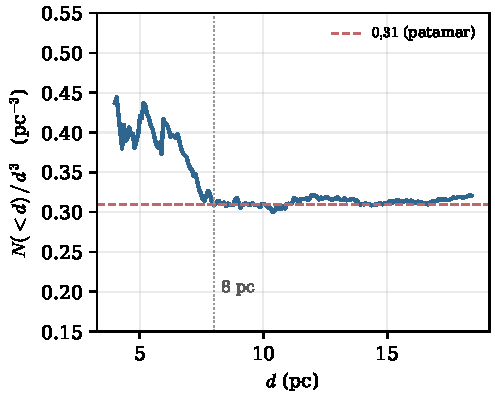
\includegraphics[width=\linewidth]{fig_completeza.pdf}
    \caption{Teste de completeza. Se a densidade for uniforme,
             $N(<d)/d^{3}$ é constante. O patamar em $0{,}31$ começa em
             $8\,\mathrm{pc}$ e vai até o limite da amostra; a subida à
             esquerda é flutuação de Poisson, não excesso real de
             estrelas.}
    \label{fig:completeza}
\end{figure}

O patamar autoriza usar $R=18{,}4\,\mathrm{pc}$ com $N=2000$. Ele também
diz algo fisicamente relevante: em uma escala de vinte parsecs a densidade
estelar é uniforme, o que é esperado, já que a altura de escala do disco
fino é de algumas centenas de parsecs.

\subsection{O diagrama cor--magnitude}

Com a Equação~\eqref{eq:modulo} calculei $M_G$ para todas as estrelas e
construí o diagrama da Figura~\ref{fig:hr}. Duas populações aparecem
separadas sem ambiguidade. A faixa diagonal é a sequência principal, que
concentra a quase totalidade da amostra. O grupo destacado no canto
inferior esquerdo --- fraco e azul ao mesmo tempo, portanto quente e
pequeno --- são anãs brancas.

Adotei como critério de separação $M_G>10$ e
$G_{\rm BP}-G_{\rm RP}<1{,}5$, escolhido por inspeção do próprio diagrama:
a linha horizontal separa as duas nuvens em luminosidade e a vertical
evita que as anãs vermelhas mais frias, que também são fracas, sejam
contadas como anãs brancas. Com esse critério há 116 anãs brancas e 1884
estrelas de sequência principal, ou $5{,}8\%\pm0{,}5\%$ do total. O
critério importa: relaxando o corte de cor para $2{,}0$ a contagem sobe
para 123, uma variação de $6\%$ --- maior que a incerteza de Poisson e
portanto uma incerteza sistemática do método, não do dado.

\begin{figure}[t]
    \centering
    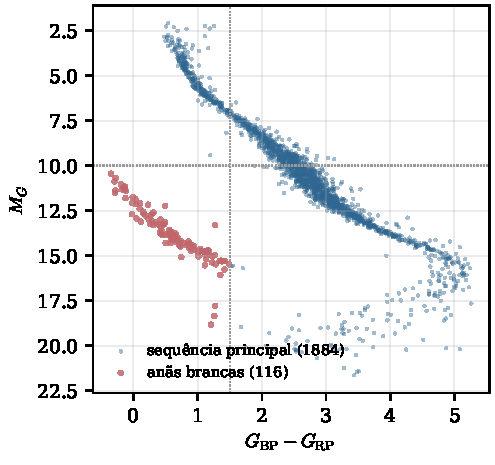
\includegraphics[width=\linewidth]{fig_hr.pdf}
    \caption{Diagrama cor--magnitude das 2000 estrelas. As linhas
             pontilhadas marcam o critério adotado para separar as duas
             populações. Note que a sequência principal se estende até
             $M_G\simeq20$: a amostra é dominada por anãs vermelhas, e o
             topo do diagrama está vazio.}
    \label{fig:hr}
\end{figure}

O topo do diagrama merece atenção: a estrela mais luminosa da amostra tem
$M_G=2{,}1$, e não há nenhuma gigante. Parte disso é real --- gigantes são
raras por unidade de volume, porque a fase de gigante dura pouco. Mas
parte é artefato: como registrado no início desta seção, Pollux, Arcturus
e Capella estão dentro de $18{,}4\,\mathrm{pc}$ e foram removidas pelo
limite de saturação. O diagrama, portanto, não pode ser
usado para estimar a fração de gigantes.

\subsection{A densidade estelar local}

Com $N=2000$ e $R=18{,}407\,\mathrm{pc}$, o volume é
$V=\tfrac{4}{3}\pi R^{3}=2{,}61\times10^{4}\,\mathrm{pc^{3}}$, e a
Equação~\eqref{eq:densidade} dá
\begin{equation}
    n = 0{,}0766 \pm 0{,}0017\ \mathrm{pc^{-3}} ,
    \label{eq:resultado}
\end{equation}
em que a incerteza é apenas estatística ($1/\sqrt{2000}=2{,}2\%$).

O censo da vizinhança solar dentro de $10\,\mathrm{pc}$, que inclui anãs
marrons e companheiras de sistemas múltiplos, reúne cerca de
$0{,}10\,\mathrm{pc^{-3}}$ \cite{recons,apostila}. O valor medido aqui
corresponde a $77\%$ desse número. A diferença, $0{,}023\,\mathrm{pc^{-3}}$,
equivale a $13{,}8$ vezes a incerteza estatística: não é flutuação, é
efeito sistemático, e vale mais discuti-lo do que lamentá-lo.

Três causas explicam o déficit, em ordem de importância estimada.
\emph{Companheiras não resolvidas.} Cerca de um terço dos sistemas da
vizinhança solar é múltiplo, e pares separados por menos de um segundo de
arco não entram no catálogo como duas fontes. \emph{Anãs marrons.} O censo
de referência as inclui; elas não são estrelas, e o \textit{Gaia} só
detecta as mais próximas e mais quentes --- por definição de amostra, esta
análise mede densidade de estrelas, não de objetos subestelares.
\emph{Saturação no extremo brilhante.} As dez a quinze estrelas mais
brilhantes do volume estão ausentes; em número são menos de $1\%$, de modo
que essa causa afeta pouco a densidade, embora arruíne qualquer estimativa
sobre gigantes.

A primeira e a segunda causas, somadas, são da ordem dos $23\%$ que
faltam, o que torna o resultado consistente com o censo de referência
\emph{depois} de reconhecido o que cada amostra conta. A conclusão
metodológica é que a incerteza dominante deste tipo de medida nunca é a
contagem: é a definição do que está sendo contado.

\subsection{Cinemática: o que os dados dizem e o que não dizem}

Apliquei a Equação~\eqref{eq:vt} a toda a amostra e obtive a velocidade
espacial para as 1439 estrelas com velocidade radial medida
(Figura~\ref{fig:velocidades}). O maior movimento próprio é o da estrela
de Barnard, $\mu=10{,}39''$ por ano a $1{,}83\,\mathrm{pc}$, o que dá
$v_t=90\,\mathrm{km\,s^{-1}}$. A distribuição de $v$ tem mediana de
$42\,\mathrm{km\,s^{-1}}$ e uma cauda: 97 estrelas ultrapassam
$100\,\mathrm{km\,s^{-1}}$, valores típicos de disco espesso e halo.

\begin{figure*}[t]
    \centering
    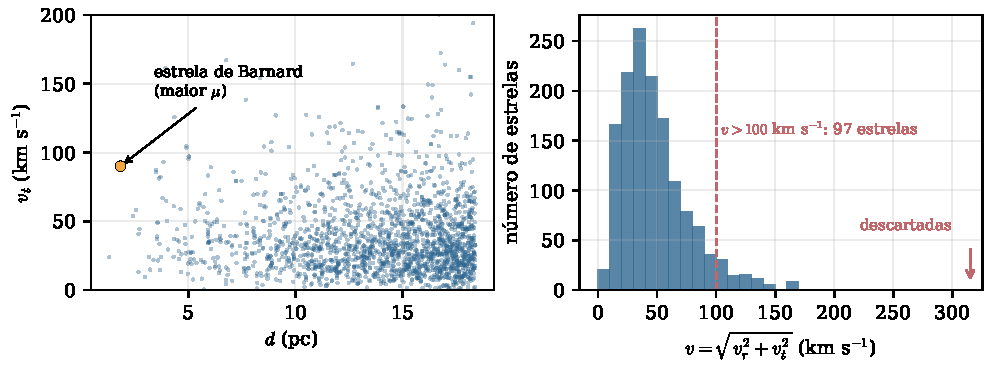
\includegraphics[width=0.92\textwidth]{fig_velocidades.pdf}
    \caption{Cinemática da amostra. \textbf{Esquerda:} velocidade
             tangencial contra distância; a ausência de pontos com $v_t$
             alto a pequena distância é efeito de seleção, porque um
             mesmo movimento próprio corresponde a $v_t$ menor quando a
             estrela está perto. \textbf{Direita:} distribuição da
             velocidade espacial das 1439 estrelas com velocidade radial
             medida. As duas medidas descartadas estão indicadas.}
    \label{fig:velocidades}
\end{figure*}

Duas estrelas, porém, não sobreviveram à verificação. Ambas aparecem no
topo da lista de velocidades, com $v_r=-414$ e
$-374\,\mathrm{km\,s^{-1}}$, mas com velocidades tangenciais de apenas
$40$ e $4\,\mathrm{km\,s^{-1}}$ --- e ambas caem na região das anãs
brancas do diagrama cor--magnitude. Para que essas medidas fossem reais, o
vetor velocidade das duas teria de estar alinhado com a linha de visada
dentro de poucos graus, duas vezes, em pouco mais de cem objetos. Além
disso, a velocidade radial espectroscópica de anãs brancas é notoriamente
difícil, porque suas linhas são largas e deslocadas pelo redshift
gravitacional. Descartei as duas medidas e registro aqui a decisão, que
não altera nenhum resultado deste artigo --- a densidade não depende da
cinemática --- mas alteraria bastante qualquer conclusão sobre a fração de
estrelas de halo na amostra.

% =====================================================================
\section{Conclusão}
\label{sec:conclusao}
% =====================================================================

A densidade estelar da vizinhança solar medida a partir das 2000 estrelas
mais próximas com paralaxe do \textit{Gaia} é
$n=0{,}0766\pm0{,}0017\ \mathrm{pc^{-3}}$
(Equação~\ref{eq:resultado}), dentro de um volume de raio
$18{,}4\,\mathrm{pc}$ cuja completeza foi verificada, e não suposta, pelo
comportamento de $N(<d)/d^{3}$.

A incerteza citada é estatística e vale $2{,}2\%$, mas ela não é a
limitação real da medida. O erro que domina é sistemático e vem da
definição da amostra: o catálogo não resolve companheiras próximas, não
inclui anãs marrons e perde as estrelas mais brilhantes. Esses três
efeitos, e não a contagem, respondem pelos $23\%$ que separam o resultado
do censo de referência. É por isso que o número medido não deve ser lido
como uma discordância: as duas contagens contam coisas diferentes, e a
comparação só é informativa depois de dito o quê.

Melhorar a medida não passa por mais estrelas nem por paralaxes melhores
--- as distâncias já têm precisão de $1\%$. Passa por resolver as
binárias próximas, o que exige imageamento de alta resolução angular ou
astrometria de longo período, e por combinar o catálogo óptico com
levantamentos no infravermelho, onde as anãs mais frias aparecem. Uma
segunda melhoria seria repetir a análise separando as populações por cor,
o que daria a função de luminosidade local em vez de um único número.

% =====================================================================
%  BIBLIOGRAFIA
% =====================================================================
\begin{thebibliography}{9}
\small

\bibitem{carroll}
CARROLL, B. W.; OSTLIE, D. A.
\textit{An Introduction to Modern Astrophysics}.
2. ed. Cambridge: Cambridge University Press, 2017.

\bibitem{apostila}
LIMA, R. C. R. de.
\textit{Astrofísica Moderna: capítulos de estudo}.
UDESC, 2026. Capítulo 1 e Laboratório de dados 1. Disponível em:
\url{https://rafaelcrdelima.github.io/Astronomia/}.

\bibitem{gaia}
GAIA COLLABORATION; VALLENARI, A. \textit{et al.}
Gaia Data Release 3: summary of the content and survey properties.
\textit{Astronomy \& Astrophysics}, v. 674, A1, 2023.

\bibitem{luri}
LURI, X. \textit{et al.}
Gaia Data Release 2: using Gaia parallaxes.
\textit{Astronomy \& Astrophysics}, v. 616, A9, 2018.

\bibitem{recons}
HENRY, T. J. \textit{et al.}
The Solar Neighborhood XLIV: RECONS discoveries within 10 parsecs.
\textit{The Astronomical Journal}, v. 155, n. 6, p. 265, 2018.

\end{thebibliography}

\end{document}
